% SOURCE: edit-harness/results/frame_a/cells/cell_*_real_MIX_{A,B,C}_*.json
% !TEX encoding = UTF-8 Unicode
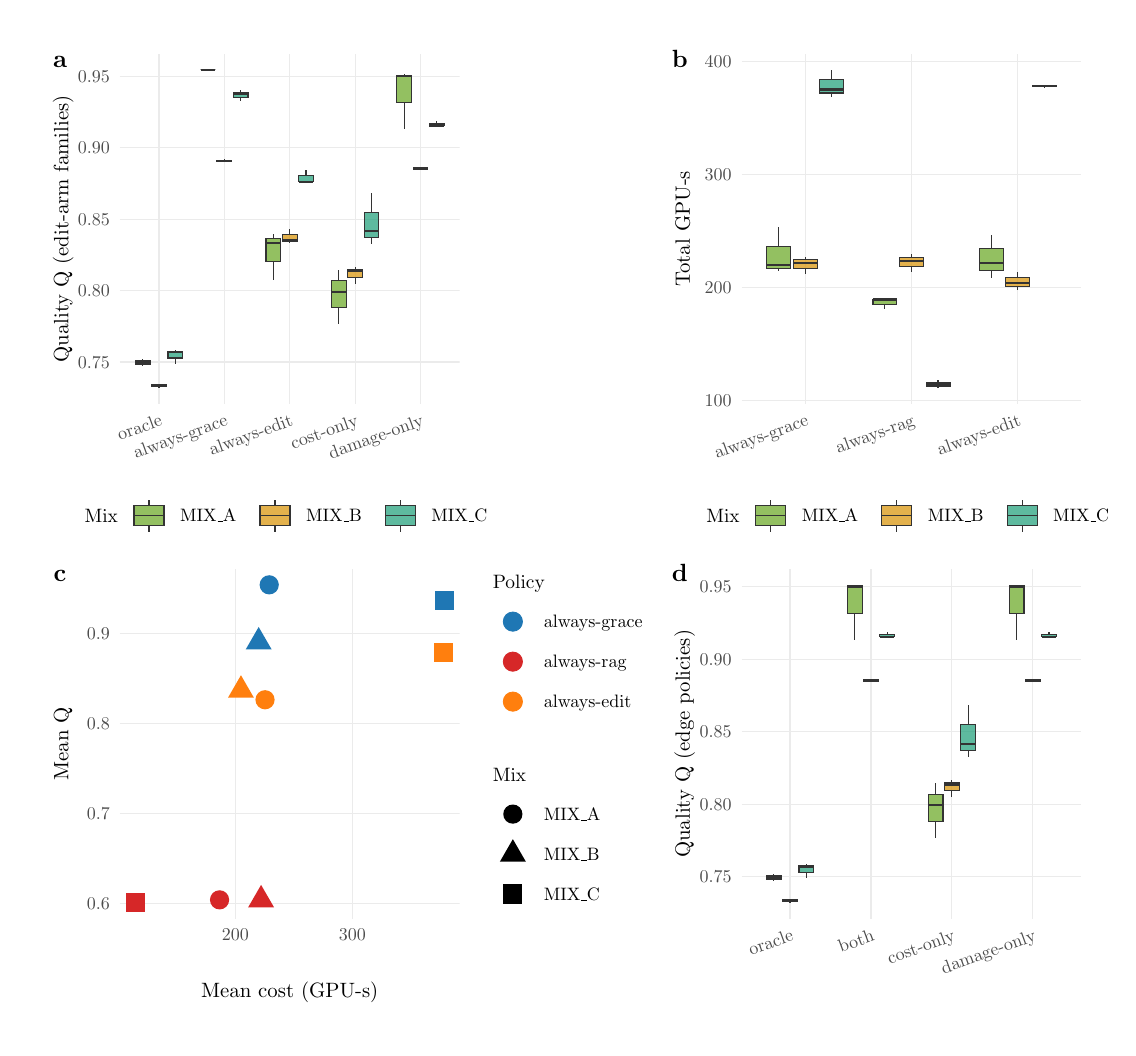
\begin{tikzpicture}[x=1pt,y=1pt]
\definecolor{fillColor}{RGB}{255,255,255}
\path[use as bounding box,fill=fillColor,fill opacity=0.00] (0,0) rectangle (390.26,361.35);
\begin{scope}
\path[clip] (  0.00,  0.00) rectangle (390.26,361.35);
\definecolor{drawColor}{RGB}{255,255,255}
\definecolor{fillColor}{RGB}{255,255,255}

\path[draw=drawColor,line width= 0.6pt,line join=round,line cap=round,fill=fillColor] (  0.00,  0.00) rectangle (390.26,361.35);
\end{scope}
\begin{scope}
\path[clip] (  5.50,169.76) rectangle (230.16,355.85);
\definecolor{fillColor}{RGB}{255,255,255}

\path[fill=fillColor] (  5.50,169.76) rectangle (230.16,355.85);
\end{scope}
\begin{scope}
\path[clip] (230.16,169.76) rectangle (384.76,355.85);
\definecolor{fillColor}{RGB}{255,255,255}

\path[fill=fillColor] (230.16,169.76) rectangle (384.76,355.85);
\end{scope}
\begin{scope}
\path[clip] (  5.50,  5.50) rectangle (230.16,169.76);
\definecolor{fillColor}{RGB}{255,255,255}

\path[fill=fillColor] (  5.50,  5.50) rectangle (230.16,169.76);
\end{scope}
\begin{scope}
\path[clip] (230.16,  5.50) rectangle (384.76,169.76);
\definecolor{fillColor}{RGB}{255,255,255}

\path[fill=fillColor] (230.16,  5.50) rectangle (384.76,169.76);
\end{scope}
\begin{scope}
\path[clip] ( 33.28,225.49) rectangle (156.09,351.85);
\definecolor{drawColor}{gray}{0.92}

\path[draw=drawColor,line width= 0.4pt,line join=round] ( 33.28,240.54) --
	(156.09,240.54);

\path[draw=drawColor,line width= 0.4pt,line join=round] ( 33.28,266.36) --
	(156.09,266.36);

\path[draw=drawColor,line width= 0.4pt,line join=round] ( 33.28,292.19) --
	(156.09,292.19);

\path[draw=drawColor,line width= 0.4pt,line join=round] ( 33.28,318.01) --
	(156.09,318.01);

\path[draw=drawColor,line width= 0.4pt,line join=round] ( 33.28,343.83) --
	(156.09,343.83);

\path[draw=drawColor,line width= 0.4pt,line join=round] ( 47.45,225.49) --
	( 47.45,351.85);

\path[draw=drawColor,line width= 0.4pt,line join=round] ( 71.07,225.49) --
	( 71.07,351.85);

\path[draw=drawColor,line width= 0.4pt,line join=round] ( 94.69,225.49) --
	( 94.69,351.85);

\path[draw=drawColor,line width= 0.4pt,line join=round] (118.30,225.49) --
	(118.30,351.85);

\path[draw=drawColor,line width= 0.4pt,line join=round] (141.92,225.49) --
	(141.92,351.85);
\definecolor{drawColor}{gray}{0.20}

\path[draw=drawColor,line width= 0.4pt,line join=round] ( 41.54,240.95) -- ( 41.54,241.57);

\path[draw=drawColor,line width= 0.4pt,line join=round] ( 41.54,239.71) -- ( 41.54,239.09);
\definecolor{fillColor}{RGB}{102,166,31}

\path[draw=drawColor,line width= 0.4pt,fill=fillColor,fill opacity=0.70] ( 38.89,240.95) --
	( 38.89,239.71) --
	( 44.20,239.71) --
	( 44.20,240.95) --
	( 38.89,240.95) --
	cycle;

\path[draw=drawColor,line width= 0.8pt] ( 38.89,240.33) -- ( 44.20,240.33);

\path[draw=drawColor,line width= 0.4pt,line join=round] ( 47.45,232.27) -- ( 47.45,232.48);

\path[draw=drawColor,line width= 0.4pt,line join=round] ( 47.45,231.65) -- ( 47.45,231.24);
\definecolor{fillColor}{RGB}{216,144,0}

\path[draw=drawColor,line width= 0.4pt,fill=fillColor,fill opacity=0.70] ( 44.79,232.27) --
	( 44.79,231.65) --
	( 50.10,231.65) --
	( 50.10,232.27) --
	( 44.79,232.27) --
	cycle;

\path[draw=drawColor,line width= 0.8pt] ( 44.79,232.06) -- ( 50.10,232.06);

\path[draw=drawColor,line width= 0.4pt,line join=round] ( 53.35,244.47) -- ( 53.35,244.88);

\path[draw=drawColor,line width= 0.4pt,line join=round] ( 53.35,241.99) -- ( 53.35,239.92);
\definecolor{fillColor}{RGB}{27,158,119}

\path[draw=drawColor,line width= 0.4pt,fill=fillColor,fill opacity=0.70] ( 50.69,244.47) --
	( 50.69,241.99) --
	( 56.01,241.99) --
	( 56.01,244.47) --
	( 50.69,244.47) --
	cycle;

\path[draw=drawColor,line width= 0.8pt] ( 50.69,244.05) -- ( 56.01,244.05);

\path[draw=drawColor,line width= 0.4pt,line join=round] ( 65.16,346.11) -- ( 65.16,346.11);

\path[draw=drawColor,line width= 0.4pt,line join=round] ( 65.16,346.11) -- ( 65.16,346.11);
\definecolor{fillColor}{RGB}{102,166,31}

\path[draw=drawColor,line width= 0.4pt,fill=fillColor,fill opacity=0.70] ( 62.50,346.11) --
	( 62.50,346.11) --
	( 67.82,346.11) --
	( 67.82,346.11) --
	( 62.50,346.11) --
	cycle;

\path[draw=drawColor,line width= 0.8pt] ( 62.50,346.11) -- ( 67.82,346.11);

\path[draw=drawColor,line width= 0.4pt,line join=round] ( 71.07,313.46) -- ( 71.07,313.87);

\path[draw=drawColor,line width= 0.4pt,line join=round] ( 71.07,313.05) -- ( 71.07,313.05);
\definecolor{fillColor}{RGB}{216,144,0}

\path[draw=drawColor,line width= 0.4pt,fill=fillColor,fill opacity=0.70] ( 68.41,313.46) --
	( 68.41,313.05) --
	( 73.72,313.05) --
	( 73.72,313.46) --
	( 68.41,313.46) --
	cycle;

\path[draw=drawColor,line width= 0.8pt] ( 68.41,313.05) -- ( 73.72,313.05);

\path[draw=drawColor,line width= 0.4pt,line join=round] ( 76.97,338.05) -- ( 76.97,338.67);

\path[draw=drawColor,line width= 0.4pt,line join=round] ( 76.97,336.19) -- ( 76.97,334.95);
\definecolor{fillColor}{RGB}{27,158,119}

\path[draw=drawColor,line width= 0.4pt,fill=fillColor,fill opacity=0.70] ( 74.31,338.05) --
	( 74.31,336.19) --
	( 79.63,336.19) --
	( 79.63,338.05) --
	( 74.31,338.05) --
	cycle;

\path[draw=drawColor,line width= 0.8pt] ( 74.31,337.43) -- ( 79.63,337.43);

\path[draw=drawColor,line width= 0.4pt,line join=round] ( 88.78,285.08) -- ( 88.78,286.73);

\path[draw=drawColor,line width= 0.4pt,line join=round] ( 88.78,276.77) -- ( 88.78,270.11);
\definecolor{fillColor}{RGB}{102,166,31}

\path[draw=drawColor,line width= 0.4pt,fill=fillColor,fill opacity=0.70] ( 86.12,285.08) --
	( 86.12,276.77) --
	( 91.44,276.77) --
	( 91.44,285.08) --
	( 86.12,285.08) --
	cycle;

\path[draw=drawColor,line width= 0.8pt] ( 86.12,283.42) -- ( 91.44,283.42);

\path[draw=drawColor,line width= 0.4pt,line join=round] ( 94.69,286.57) -- ( 94.69,288.65);

\path[draw=drawColor,line width= 0.4pt,line join=round] ( 94.69,284.06) -- ( 94.69,283.61);
\definecolor{fillColor}{RGB}{216,144,0}

\path[draw=drawColor,line width= 0.4pt,fill=fillColor,fill opacity=0.70] ( 92.03,286.57) --
	( 92.03,284.06) --
	( 97.34,284.06) --
	( 97.34,286.57) --
	( 92.03,286.57) --
	cycle;

\path[draw=drawColor,line width= 0.8pt] ( 92.03,284.50) -- ( 97.34,284.50);

\path[draw=drawColor,line width= 0.4pt,line join=round] (100.59,307.90) -- (100.59,310.08);

\path[draw=drawColor,line width= 0.4pt,line join=round] (100.59,305.64) -- (100.59,305.57);
\definecolor{fillColor}{RGB}{27,158,119}

\path[draw=drawColor,line width= 0.4pt,fill=fillColor,fill opacity=0.70] ( 97.93,307.90) --
	( 97.93,305.64) --
	(103.25,305.64) --
	(103.25,307.90) --
	( 97.93,307.90) --
	cycle;

\path[draw=drawColor,line width= 0.8pt] ( 97.93,305.72) -- (103.25,305.72);

\path[draw=drawColor,line width= 0.4pt,line join=round] (112.40,269.91) -- (112.40,273.90);

\path[draw=drawColor,line width= 0.4pt,line join=round] (112.40,260.17) -- (112.40,254.40);
\definecolor{fillColor}{RGB}{102,166,31}

\path[draw=drawColor,line width= 0.4pt,fill=fillColor,fill opacity=0.70] (109.74,269.91) --
	(109.74,260.17) --
	(115.06,260.17) --
	(115.06,269.91) --
	(109.74,269.91) --
	cycle;

\path[draw=drawColor,line width= 0.8pt] (109.74,265.93) -- (115.06,265.93);

\path[draw=drawColor,line width= 0.4pt,line join=round] (118.30,274.09) -- (118.30,274.84);

\path[draw=drawColor,line width= 0.4pt,line join=round] (118.30,271.07) -- (118.30,268.80);
\definecolor{fillColor}{RGB}{216,144,0}

\path[draw=drawColor,line width= 0.4pt,fill=fillColor,fill opacity=0.70] (115.65,274.09) --
	(115.65,271.07) --
	(120.96,271.07) --
	(120.96,274.09) --
	(115.65,274.09) --
	cycle;

\path[draw=drawColor,line width= 0.8pt] (115.65,273.34) -- (120.96,273.34);

\path[draw=drawColor,line width= 0.4pt,line join=round] (124.21,294.72) -- (124.21,301.65);

\path[draw=drawColor,line width= 0.4pt,line join=round] (124.21,285.52) -- (124.21,283.25);
\definecolor{fillColor}{RGB}{27,158,119}

\path[draw=drawColor,line width= 0.4pt,fill=fillColor,fill opacity=0.70] (121.55,294.72) --
	(121.55,285.52) --
	(126.87,285.52) --
	(126.87,294.72) --
	(121.55,294.72) --
	cycle;

\path[draw=drawColor,line width= 0.8pt] (121.55,287.78) -- (126.87,287.78);

\path[draw=drawColor,line width= 0.4pt,line join=round] (136.02,344.22) -- (136.02,344.51);

\path[draw=drawColor,line width= 0.4pt,line join=round] (136.02,334.41) -- (136.02,324.91);
\definecolor{fillColor}{RGB}{102,166,31}

\path[draw=drawColor,line width= 0.4pt,fill=fillColor,fill opacity=0.70] (133.36,344.22) --
	(133.36,334.41) --
	(138.68,334.41) --
	(138.68,344.22) --
	(133.36,344.22) --
	cycle;

\path[draw=drawColor,line width= 0.8pt] (133.36,343.92) -- (138.68,343.92);

\path[draw=drawColor,line width= 0.4pt,line join=round] (141.92,310.64) -- (141.92,310.99);

\path[draw=drawColor,line width= 0.4pt,line join=round] (141.92,310.12) -- (141.92,309.97);
\definecolor{fillColor}{RGB}{216,144,0}

\path[draw=drawColor,line width= 0.4pt,fill=fillColor,fill opacity=0.70] (139.27,310.64) --
	(139.27,310.12) --
	(144.58,310.12) --
	(144.58,310.64) --
	(139.27,310.64) --
	cycle;

\path[draw=drawColor,line width= 0.8pt] (139.27,310.28) -- (144.58,310.28);

\path[draw=drawColor,line width= 0.4pt,line join=round] (147.83,326.78) -- (147.83,327.59);

\path[draw=drawColor,line width= 0.4pt,line join=round] (147.83,325.96) -- (147.83,325.93);
\definecolor{fillColor}{RGB}{27,158,119}

\path[draw=drawColor,line width= 0.4pt,fill=fillColor,fill opacity=0.70] (145.17,326.78) --
	(145.17,325.96) --
	(150.49,325.96) --
	(150.49,326.78) --
	(145.17,326.78) --
	cycle;

\path[draw=drawColor,line width= 0.8pt] (145.17,325.98) -- (150.49,325.98);
\end{scope}
\begin{scope}
\path[clip] (  0.00,  0.00) rectangle (390.26,361.35);
\definecolor{drawColor}{gray}{0.30}

\node[text=drawColor,anchor=base east,inner sep=0pt, outer sep=0pt, scale=  0.65] at ( 29.68,238.30) {0.75};

\node[text=drawColor,anchor=base east,inner sep=0pt, outer sep=0pt, scale=  0.65] at ( 29.68,264.13) {0.80};

\node[text=drawColor,anchor=base east,inner sep=0pt, outer sep=0pt, scale=  0.65] at ( 29.68,289.95) {0.85};

\node[text=drawColor,anchor=base east,inner sep=0pt, outer sep=0pt, scale=  0.65] at ( 29.68,315.77) {0.90};

\node[text=drawColor,anchor=base east,inner sep=0pt, outer sep=0pt, scale=  0.65] at ( 29.68,341.60) {0.95};
\end{scope}
\begin{scope}
\path[clip] (  0.00,  0.00) rectangle (390.26,361.35);
\definecolor{drawColor}{gray}{0.30}

\node[text=drawColor,rotate= 20.00,anchor=base east,inner sep=0pt, outer sep=0pt, scale=  0.65] at ( 48.98,217.69) {oracle};

\node[text=drawColor,rotate= 20.00,anchor=base east,inner sep=0pt, outer sep=0pt, scale=  0.65] at ( 72.60,217.69) {always-grace};

\node[text=drawColor,rotate= 20.00,anchor=base east,inner sep=0pt, outer sep=0pt, scale=  0.65] at ( 96.22,217.69) {always-edit};

\node[text=drawColor,rotate= 20.00,anchor=base east,inner sep=0pt, outer sep=0pt, scale=  0.65] at (119.84,217.69) {cost-only};

\node[text=drawColor,rotate= 20.00,anchor=base east,inner sep=0pt, outer sep=0pt, scale=  0.65] at (143.45,217.69) {damage-only};
\end{scope}
\begin{scope}
\path[clip] (  0.00,  0.00) rectangle (390.26,361.35);
\definecolor{drawColor}{RGB}{0,0,0}

\node[text=drawColor,rotate= 90.00,anchor=base,inner sep=0pt, outer sep=0pt, scale=  0.75] at ( 14.67,288.67) {Quality Q (edit-arm families)};
\end{scope}
\begin{scope}
\path[clip] (  0.00,  0.00) rectangle (390.26,361.35);
\definecolor{drawColor}{RGB}{0,0,0}

\node[text=drawColor,anchor=base west,inner sep=0pt, outer sep=0pt, scale=  0.70] at ( 20.55,182.58) {Mix};
\end{scope}
\begin{scope}
\path[clip] (  0.00,  0.00) rectangle (390.26,361.35);
\definecolor{drawColor}{gray}{0.20}

\path[draw=drawColor,line width= 0.4pt] ( 43.83,179.21) --
	( 43.83,181.37);

\path[draw=drawColor,line width= 0.4pt] ( 43.83,188.60) --
	( 43.83,190.77);
\definecolor{fillColor}{RGB}{102,166,31}

\path[draw=drawColor,line width= 0.4pt,fill=fillColor,fill opacity=0.70] ( 38.41,181.37) rectangle ( 49.25,188.60);

\path[draw=drawColor,line width= 0.4pt] ( 38.41,184.99) --
	( 49.25,184.99);

\path[draw=drawColor,line width= 0.4pt] ( 43.83,179.21) --
	( 43.83,179.21);

\path[draw=drawColor,line width= 0.4pt] ( 43.83,190.77) --
	( 43.83,190.77);
\end{scope}
\begin{scope}
\path[clip] (  0.00,  0.00) rectangle (390.26,361.35);
\definecolor{drawColor}{gray}{0.20}

\path[draw=drawColor,line width= 0.4pt] ( 89.38,179.21) --
	( 89.38,181.37);

\path[draw=drawColor,line width= 0.4pt] ( 89.38,188.60) --
	( 89.38,190.77);
\definecolor{fillColor}{RGB}{216,144,0}

\path[draw=drawColor,line width= 0.4pt,fill=fillColor,fill opacity=0.70] ( 83.96,181.37) rectangle ( 94.80,188.60);

\path[draw=drawColor,line width= 0.4pt] ( 83.96,184.99) --
	( 94.80,184.99);

\path[draw=drawColor,line width= 0.4pt] ( 89.38,179.21) --
	( 89.38,179.21);

\path[draw=drawColor,line width= 0.4pt] ( 89.38,190.77) --
	( 89.38,190.77);
\end{scope}
\begin{scope}
\path[clip] (  0.00,  0.00) rectangle (390.26,361.35);
\definecolor{drawColor}{gray}{0.20}

\path[draw=drawColor,line width= 0.4pt] (134.67,179.21) --
	(134.67,181.37);

\path[draw=drawColor,line width= 0.4pt] (134.67,188.60) --
	(134.67,190.77);
\definecolor{fillColor}{RGB}{27,158,119}

\path[draw=drawColor,line width= 0.4pt,fill=fillColor,fill opacity=0.70] (129.25,181.37) rectangle (140.09,188.60);

\path[draw=drawColor,line width= 0.4pt] (129.25,184.99) --
	(140.09,184.99);

\path[draw=drawColor,line width= 0.4pt] (134.67,179.21) --
	(134.67,179.21);

\path[draw=drawColor,line width= 0.4pt] (134.67,190.77) --
	(134.67,190.77);
\end{scope}
\begin{scope}
\path[clip] (  0.00,  0.00) rectangle (390.26,361.35);
\definecolor{drawColor}{RGB}{0,0,0}

\node[text=drawColor,anchor=base west,inner sep=0pt, outer sep=0pt, scale=  0.65] at ( 55.05,182.75) {MIX\_A};
\end{scope}
\begin{scope}
\path[clip] (  0.00,  0.00) rectangle (390.26,361.35);
\definecolor{drawColor}{RGB}{0,0,0}

\node[text=drawColor,anchor=base west,inner sep=0pt, outer sep=0pt, scale=  0.65] at (100.61,182.75) {MIX\_B};
\end{scope}
\begin{scope}
\path[clip] (  0.00,  0.00) rectangle (390.26,361.35);
\definecolor{drawColor}{RGB}{0,0,0}

\node[text=drawColor,anchor=base west,inner sep=0pt, outer sep=0pt, scale=  0.65] at (145.90,182.75) {MIX\_C};
\end{scope}
\begin{scope}
\path[clip] (  0.00,  0.00) rectangle (390.26,361.35);
\definecolor{drawColor}{RGB}{0,0,0}

\node[text=drawColor,anchor=base,inner sep=0pt, outer sep=0pt, scale=  0.90] at ( 11.67,346.96) {\bfseries a};
\end{scope}
\begin{scope}
\path[clip] (257.94,225.49) rectangle (380.76,351.85);
\definecolor{drawColor}{gray}{0.92}

\path[draw=drawColor,line width= 0.4pt,line join=round] (257.94,226.66) --
	(380.76,226.66);

\path[draw=drawColor,line width= 0.4pt,line join=round] (257.94,267.53) --
	(380.76,267.53);

\path[draw=drawColor,line width= 0.4pt,line join=round] (257.94,308.40) --
	(380.76,308.40);

\path[draw=drawColor,line width= 0.4pt,line join=round] (257.94,349.27) --
	(380.76,349.27);

\path[draw=drawColor,line width= 0.4pt,line join=round] (280.97,225.49) --
	(280.97,351.85);

\path[draw=drawColor,line width= 0.4pt,line join=round] (319.35,225.49) --
	(319.35,351.85);

\path[draw=drawColor,line width= 0.4pt,line join=round] (357.73,225.49) --
	(357.73,351.85);
\definecolor{drawColor}{gray}{0.20}

\path[draw=drawColor,line width= 0.4pt,line join=round] (271.37,282.35) -- (271.37,289.25);

\path[draw=drawColor,line width= 0.4pt,line join=round] (271.37,274.46) -- (271.37,273.46);
\definecolor{fillColor}{RGB}{102,166,31}

\path[draw=drawColor,line width= 0.4pt,fill=fillColor,fill opacity=0.70] (267.05,282.35) --
	(267.05,274.46) --
	(275.69,274.46) --
	(275.69,282.35) --
	(267.05,282.35) --
	cycle;

\path[draw=drawColor,line width= 0.8pt] (267.05,275.45) -- (275.69,275.45);

\path[draw=drawColor,line width= 0.4pt,line join=round] (280.97,277.42) -- (280.97,278.46);

\path[draw=drawColor,line width= 0.4pt,line join=round] (280.97,274.33) -- (280.97,272.27);
\definecolor{fillColor}{RGB}{216,144,0}

\path[draw=drawColor,line width= 0.4pt,fill=fillColor,fill opacity=0.70] (276.65,277.42) --
	(276.65,274.33) --
	(285.29,274.33) --
	(285.29,277.42) --
	(276.65,277.42) --
	cycle;

\path[draw=drawColor,line width= 0.8pt] (276.65,276.39) -- (285.29,276.39);

\path[draw=drawColor,line width= 0.4pt,line join=round] (290.56,342.55) -- (290.56,346.11);

\path[draw=drawColor,line width= 0.4pt,line join=round] (290.56,337.73) -- (290.56,336.47);
\definecolor{fillColor}{RGB}{27,158,119}

\path[draw=drawColor,line width= 0.4pt,fill=fillColor,fill opacity=0.70] (286.25,342.55) --
	(286.25,337.73) --
	(294.88,337.73) --
	(294.88,342.55) --
	(286.25,342.55) --
	cycle;

\path[draw=drawColor,line width= 0.8pt] (286.25,338.99) -- (294.88,338.99);

\path[draw=drawColor,line width= 0.4pt,line join=round] (309.75,263.20) -- (309.75,263.27);

\path[draw=drawColor,line width= 0.4pt,line join=round] (309.75,261.43) -- (309.75,259.72);
\definecolor{fillColor}{RGB}{102,166,31}

\path[draw=drawColor,line width= 0.4pt,fill=fillColor,fill opacity=0.70] (305.44,263.20) --
	(305.44,261.43) --
	(314.07,261.43) --
	(314.07,263.20) --
	(305.44,263.20) --
	cycle;

\path[draw=drawColor,line width= 0.8pt] (305.44,263.14) -- (314.07,263.14);

\path[draw=drawColor,line width= 0.4pt,line join=round] (319.35,278.21) -- (319.35,279.48);

\path[draw=drawColor,line width= 0.4pt,line join=round] (319.35,275.08) -- (319.35,273.22);
\definecolor{fillColor}{RGB}{216,144,0}

\path[draw=drawColor,line width= 0.4pt,fill=fillColor,fill opacity=0.70] (315.03,278.21) --
	(315.03,275.08) --
	(323.67,275.08) --
	(323.67,278.21) --
	(315.03,278.21) --
	cycle;

\path[draw=drawColor,line width= 0.8pt] (315.03,276.94) -- (323.67,276.94);

\path[draw=drawColor,line width= 0.4pt,line join=round] (328.94,233.23) -- (328.94,234.04);

\path[draw=drawColor,line width= 0.4pt,line join=round] (328.94,231.83) -- (328.94,231.24);
\definecolor{fillColor}{RGB}{27,158,119}

\path[draw=drawColor,line width= 0.4pt,fill=fillColor,fill opacity=0.70] (324.63,233.23) --
	(324.63,231.83) --
	(333.26,231.83) --
	(333.26,233.23) --
	(324.63,233.23) --
	cycle;

\path[draw=drawColor,line width= 0.8pt] (324.63,232.43) -- (333.26,232.43);

\path[draw=drawColor,line width= 0.4pt,line join=round] (348.13,281.49) -- (348.13,286.52);

\path[draw=drawColor,line width= 0.4pt,line join=round] (348.13,273.62) -- (348.13,270.79);
\definecolor{fillColor}{RGB}{102,166,31}

\path[draw=drawColor,line width= 0.4pt,fill=fillColor,fill opacity=0.70] (343.82,281.49) --
	(343.82,273.62) --
	(352.45,273.62) --
	(352.45,281.49) --
	(343.82,281.49) --
	cycle;

\path[draw=drawColor,line width= 0.8pt] (343.82,276.45) -- (352.45,276.45);

\path[draw=drawColor,line width= 0.4pt,line join=round] (357.73,270.98) -- (357.73,272.90);

\path[draw=drawColor,line width= 0.4pt,line join=round] (357.73,267.82) -- (357.73,266.57);
\definecolor{fillColor}{RGB}{216,144,0}

\path[draw=drawColor,line width= 0.4pt,fill=fillColor,fill opacity=0.70] (353.41,270.98) --
	(353.41,267.82) --
	(362.05,267.82) --
	(362.05,270.98) --
	(353.41,270.98) --
	cycle;

\path[draw=drawColor,line width= 0.8pt] (353.41,269.07) -- (362.05,269.07);

\path[draw=drawColor,line width= 0.4pt,line join=round] (367.32,340.59) -- (367.32,340.77);

\path[draw=drawColor,line width= 0.4pt,line join=round] (367.32,339.98) -- (367.32,339.55);
\definecolor{fillColor}{RGB}{27,158,119}

\path[draw=drawColor,line width= 0.4pt,fill=fillColor,fill opacity=0.70] (363.01,340.59) --
	(363.01,339.98) --
	(371.64,339.98) --
	(371.64,340.59) --
	(363.01,340.59) --
	cycle;

\path[draw=drawColor,line width= 0.8pt] (363.01,340.41) -- (371.64,340.41);
\end{scope}
\begin{scope}
\path[clip] (  0.00,  0.00) rectangle (390.26,361.35);
\definecolor{drawColor}{gray}{0.30}

\node[text=drawColor,anchor=base east,inner sep=0pt, outer sep=0pt, scale=  0.65] at (254.34,224.42) {100};

\node[text=drawColor,anchor=base east,inner sep=0pt, outer sep=0pt, scale=  0.65] at (254.34,265.29) {200};

\node[text=drawColor,anchor=base east,inner sep=0pt, outer sep=0pt, scale=  0.65] at (254.34,306.16) {300};

\node[text=drawColor,anchor=base east,inner sep=0pt, outer sep=0pt, scale=  0.65] at (254.34,347.03) {400};
\end{scope}
\begin{scope}
\path[clip] (  0.00,  0.00) rectangle (390.26,361.35);
\definecolor{drawColor}{gray}{0.30}

\node[text=drawColor,rotate= 20.00,anchor=base east,inner sep=0pt, outer sep=0pt, scale=  0.65] at (282.50,217.69) {always-grace};

\node[text=drawColor,rotate= 20.00,anchor=base east,inner sep=0pt, outer sep=0pt, scale=  0.65] at (320.88,217.69) {always-rag};

\node[text=drawColor,rotate= 20.00,anchor=base east,inner sep=0pt, outer sep=0pt, scale=  0.65] at (359.26,217.69) {always-edit};
\end{scope}
\begin{scope}
\path[clip] (  0.00,  0.00) rectangle (390.26,361.35);
\definecolor{drawColor}{RGB}{0,0,0}

\node[text=drawColor,rotate= 90.00,anchor=base,inner sep=0pt, outer sep=0pt, scale=  0.75] at (239.33,288.67) {Total GPU-s};
\end{scope}
\begin{scope}
\path[clip] (  0.00,  0.00) rectangle (390.26,361.35);
\definecolor{drawColor}{RGB}{0,0,0}

\node[text=drawColor,anchor=base west,inner sep=0pt, outer sep=0pt, scale=  0.70] at (245.21,182.58) {Mix};
\end{scope}
\begin{scope}
\path[clip] (  0.00,  0.00) rectangle (390.26,361.35);
\definecolor{drawColor}{gray}{0.20}

\path[draw=drawColor,line width= 0.4pt] (268.49,179.21) --
	(268.49,181.37);

\path[draw=drawColor,line width= 0.4pt] (268.49,188.60) --
	(268.49,190.77);
\definecolor{fillColor}{RGB}{102,166,31}

\path[draw=drawColor,line width= 0.4pt,fill=fillColor,fill opacity=0.70] (263.07,181.37) rectangle (273.91,188.60);

\path[draw=drawColor,line width= 0.4pt] (263.07,184.99) --
	(273.91,184.99);

\path[draw=drawColor,line width= 0.4pt] (268.49,179.21) --
	(268.49,179.21);

\path[draw=drawColor,line width= 0.4pt] (268.49,190.77) --
	(268.49,190.77);
\end{scope}
\begin{scope}
\path[clip] (  0.00,  0.00) rectangle (390.26,361.35);
\definecolor{drawColor}{gray}{0.20}

\path[draw=drawColor,line width= 0.4pt] (314.05,179.21) --
	(314.05,181.37);

\path[draw=drawColor,line width= 0.4pt] (314.05,188.60) --
	(314.05,190.77);
\definecolor{fillColor}{RGB}{216,144,0}

\path[draw=drawColor,line width= 0.4pt,fill=fillColor,fill opacity=0.70] (308.63,181.37) rectangle (319.47,188.60);

\path[draw=drawColor,line width= 0.4pt] (308.63,184.99) --
	(319.47,184.99);

\path[draw=drawColor,line width= 0.4pt] (314.05,179.21) --
	(314.05,179.21);

\path[draw=drawColor,line width= 0.4pt] (314.05,190.77) --
	(314.05,190.77);
\end{scope}
\begin{scope}
\path[clip] (  0.00,  0.00) rectangle (390.26,361.35);
\definecolor{drawColor}{gray}{0.20}

\path[draw=drawColor,line width= 0.4pt] (359.34,179.21) --
	(359.34,181.37);

\path[draw=drawColor,line width= 0.4pt] (359.34,188.60) --
	(359.34,190.77);
\definecolor{fillColor}{RGB}{27,158,119}

\path[draw=drawColor,line width= 0.4pt,fill=fillColor,fill opacity=0.70] (353.92,181.37) rectangle (364.76,188.60);

\path[draw=drawColor,line width= 0.4pt] (353.92,184.99) --
	(364.76,184.99);

\path[draw=drawColor,line width= 0.4pt] (359.34,179.21) --
	(359.34,179.21);

\path[draw=drawColor,line width= 0.4pt] (359.34,190.77) --
	(359.34,190.77);
\end{scope}
\begin{scope}
\path[clip] (  0.00,  0.00) rectangle (390.26,361.35);
\definecolor{drawColor}{RGB}{0,0,0}

\node[text=drawColor,anchor=base west,inner sep=0pt, outer sep=0pt, scale=  0.65] at (279.72,182.75) {MIX\_A};
\end{scope}
\begin{scope}
\path[clip] (  0.00,  0.00) rectangle (390.26,361.35);
\definecolor{drawColor}{RGB}{0,0,0}

\node[text=drawColor,anchor=base west,inner sep=0pt, outer sep=0pt, scale=  0.65] at (325.27,182.75) {MIX\_B};
\end{scope}
\begin{scope}
\path[clip] (  0.00,  0.00) rectangle (390.26,361.35);
\definecolor{drawColor}{RGB}{0,0,0}

\node[text=drawColor,anchor=base west,inner sep=0pt, outer sep=0pt, scale=  0.65] at (370.56,182.75) {MIX\_C};
\end{scope}
\begin{scope}
\path[clip] (  0.00,  0.00) rectangle (390.26,361.35);
\definecolor{drawColor}{RGB}{0,0,0}

\node[text=drawColor,anchor=base,inner sep=0pt, outer sep=0pt, scale=  0.90] at (235.63,346.96) {\bfseries b};
\end{scope}
\begin{scope}
\path[clip] ( 33.28, 39.40) rectangle (156.09,165.76);
\definecolor{drawColor}{gray}{0.92}

\path[draw=drawColor,line width= 0.4pt,line join=round] ( 33.28, 44.89) --
	(156.09, 44.89);

\path[draw=drawColor,line width= 0.4pt,line join=round] ( 33.28, 77.37) --
	(156.09, 77.37);

\path[draw=drawColor,line width= 0.4pt,line join=round] ( 33.28,109.86) --
	(156.09,109.86);

\path[draw=drawColor,line width= 0.4pt,line join=round] ( 33.28,142.34) --
	(156.09,142.34);

\path[draw=drawColor,line width= 0.4pt,line join=round] ( 75.02, 39.40) --
	( 75.02,165.76);

\path[draw=drawColor,line width= 0.4pt,line join=round] (117.29, 39.40) --
	(117.29,165.76);
\definecolor{fillColor}{RGB}{31,119,180}

\path[fill=fillColor] ( 87.28,160.02) circle (  3.47);
\definecolor{fillColor}{RGB}{214,39,40}

\path[fill=fillColor] ( 69.34, 46.19) circle (  3.47);
\definecolor{fillColor}{RGB}{255,127,14}

\path[fill=fillColor] ( 85.77,118.49) circle (  3.47);
\definecolor{fillColor}{RGB}{31,119,180}

\path[fill=fillColor] ( 83.47,144.79) --
	( 88.15,136.69) --
	( 78.80,136.69) --
	cycle;
\definecolor{fillColor}{RGB}{214,39,40}

\path[fill=fillColor] ( 84.34, 51.59) --
	( 89.02, 43.49) --
	( 79.67, 43.49) --
	cycle;
\definecolor{fillColor}{RGB}{255,127,14}

\path[fill=fillColor] ( 77.07,127.35) --
	( 81.74,119.25) --
	( 72.39,119.25) --
	cycle;
\definecolor{fillColor}{RGB}{31,119,180}

\path[fill=fillColor] (147.04,150.83) --
	(153.98,150.83) --
	(153.98,157.77) --
	(147.04,157.77) --
	cycle;
\definecolor{fillColor}{RGB}{214,39,40}

\path[fill=fillColor] ( 35.39, 41.68) --
	( 42.33, 41.68) --
	( 42.33, 48.62) --
	( 35.39, 48.62) --
	cycle;
\definecolor{fillColor}{RGB}{255,127,14}

\path[fill=fillColor] (146.75,132.02) --
	(153.69,132.02) --
	(153.69,138.97) --
	(146.75,138.97) --
	cycle;
\end{scope}
\begin{scope}
\path[clip] (  0.00,  0.00) rectangle (390.26,361.35);
\definecolor{drawColor}{gray}{0.30}

\node[text=drawColor,anchor=base east,inner sep=0pt, outer sep=0pt, scale=  0.65] at ( 29.68, 42.65) {0.6};

\node[text=drawColor,anchor=base east,inner sep=0pt, outer sep=0pt, scale=  0.65] at ( 29.68, 75.13) {0.7};

\node[text=drawColor,anchor=base east,inner sep=0pt, outer sep=0pt, scale=  0.65] at ( 29.68,107.62) {0.8};

\node[text=drawColor,anchor=base east,inner sep=0pt, outer sep=0pt, scale=  0.65] at ( 29.68,140.11) {0.9};
\end{scope}
\begin{scope}
\path[clip] (  0.00,  0.00) rectangle (390.26,361.35);
\definecolor{drawColor}{gray}{0.30}

\node[text=drawColor,anchor=base,inner sep=0pt, outer sep=0pt, scale=  0.65] at ( 75.02, 31.33) {200};

\node[text=drawColor,anchor=base,inner sep=0pt, outer sep=0pt, scale=  0.65] at (117.29, 31.33) {300};
\end{scope}
\begin{scope}
\path[clip] (  0.00,  0.00) rectangle (390.26,361.35);
\definecolor{drawColor}{RGB}{0,0,0}

\node[text=drawColor,anchor=base,inner sep=0pt, outer sep=0pt, scale=  0.75] at ( 94.69, 10.96) {Mean cost (GPU-s)};
\end{scope}
\begin{scope}
\path[clip] (  0.00,  0.00) rectangle (390.26,361.35);
\definecolor{drawColor}{RGB}{0,0,0}

\node[text=drawColor,rotate= 90.00,anchor=base,inner sep=0pt, outer sep=0pt, scale=  0.75] at ( 14.67,102.58) {Mean Q};
\end{scope}
\begin{scope}
\path[clip] (  0.00,  0.00) rectangle (390.26,361.35);
\definecolor{drawColor}{RGB}{0,0,0}

\node[text=drawColor,anchor=base west,inner sep=0pt, outer sep=0pt, scale=  0.70] at (168.09,158.62) {Policy};
\end{scope}
\begin{scope}
\path[clip] (  0.00,  0.00) rectangle (390.26,361.35);
\definecolor{drawColor}{RGB}{31,119,180}
\definecolor{fillColor}{RGB}{31,119,180}

\path[draw=drawColor,line width= 0.3pt,line join=round,line cap=round,fill=fillColor] (175.32,146.72) circle (  3.47);
\end{scope}
\begin{scope}
\path[clip] (  0.00,  0.00) rectangle (390.26,361.35);
\definecolor{drawColor}{RGB}{214,39,40}
\definecolor{fillColor}{RGB}{214,39,40}

\path[draw=drawColor,line width= 0.3pt,line join=round,line cap=round,fill=fillColor] (175.32,132.26) circle (  3.47);
\end{scope}
\begin{scope}
\path[clip] (  0.00,  0.00) rectangle (390.26,361.35);
\definecolor{drawColor}{RGB}{255,127,14}
\definecolor{fillColor}{RGB}{255,127,14}

\path[draw=drawColor,line width= 0.3pt,line join=round,line cap=round,fill=fillColor] (175.32,117.81) circle (  3.47);
\end{scope}
\begin{scope}
\path[clip] (  0.00,  0.00) rectangle (390.26,361.35);
\definecolor{drawColor}{RGB}{0,0,0}

\node[text=drawColor,anchor=base west,inner sep=0pt, outer sep=0pt, scale=  0.65] at (186.55,144.48) {always-grace};
\end{scope}
\begin{scope}
\path[clip] (  0.00,  0.00) rectangle (390.26,361.35);
\definecolor{drawColor}{RGB}{0,0,0}

\node[text=drawColor,anchor=base west,inner sep=0pt, outer sep=0pt, scale=  0.65] at (186.55,130.02) {always-rag};
\end{scope}
\begin{scope}
\path[clip] (  0.00,  0.00) rectangle (390.26,361.35);
\definecolor{drawColor}{RGB}{0,0,0}

\node[text=drawColor,anchor=base west,inner sep=0pt, outer sep=0pt, scale=  0.65] at (186.55,115.57) {always-edit};
\end{scope}
\begin{scope}
\path[clip] (  0.00,  0.00) rectangle (390.26,361.35);
\definecolor{drawColor}{RGB}{0,0,0}

\node[text=drawColor,anchor=base west,inner sep=0pt, outer sep=0pt, scale=  0.70] at (168.09, 89.08) {Mix};
\end{scope}
\begin{scope}
\path[clip] (  0.00,  0.00) rectangle (390.26,361.35);
\definecolor{fillColor}{RGB}{0,0,0}

\path[fill=fillColor] (175.32, 77.17) circle (  3.47);
\end{scope}
\begin{scope}
\path[clip] (  0.00,  0.00) rectangle (390.26,361.35);
\definecolor{fillColor}{RGB}{0,0,0}

\path[fill=fillColor] (175.32, 68.12) --
	(180.00, 60.02) --
	(170.65, 60.02) --
	cycle;
\end{scope}
\begin{scope}
\path[clip] (  0.00,  0.00) rectangle (390.26,361.35);
\definecolor{fillColor}{RGB}{0,0,0}

\path[fill=fillColor] (171.85, 44.79) --
	(178.79, 44.79) --
	(178.79, 51.74) --
	(171.85, 51.74) --
	cycle;
\end{scope}
\begin{scope}
\path[clip] (  0.00,  0.00) rectangle (390.26,361.35);
\definecolor{drawColor}{RGB}{0,0,0}

\node[text=drawColor,anchor=base west,inner sep=0pt, outer sep=0pt, scale=  0.65] at (186.55, 74.93) {MIX\_A};
\end{scope}
\begin{scope}
\path[clip] (  0.00,  0.00) rectangle (390.26,361.35);
\definecolor{drawColor}{RGB}{0,0,0}

\node[text=drawColor,anchor=base west,inner sep=0pt, outer sep=0pt, scale=  0.65] at (186.55, 60.48) {MIX\_B};
\end{scope}
\begin{scope}
\path[clip] (  0.00,  0.00) rectangle (390.26,361.35);
\definecolor{drawColor}{RGB}{0,0,0}

\node[text=drawColor,anchor=base west,inner sep=0pt, outer sep=0pt, scale=  0.65] at (186.55, 46.03) {MIX\_C};
\end{scope}
\begin{scope}
\path[clip] (  0.00,  0.00) rectangle (390.26,361.35);
\definecolor{drawColor}{RGB}{0,0,0}

\node[text=drawColor,anchor=base,inner sep=0pt, outer sep=0pt, scale=  0.90] at ( 11.67,161.09) {\bfseries c};
\end{scope}
\begin{scope}
\path[clip] (257.94, 39.40) rectangle (380.76,165.76);
\definecolor{drawColor}{gray}{0.92}

\path[draw=drawColor,line width= 0.4pt,line join=round] (257.94, 54.58) --
	(380.76, 54.58);

\path[draw=drawColor,line width= 0.4pt,line join=round] (257.94, 80.77) --
	(380.76, 80.77);

\path[draw=drawColor,line width= 0.4pt,line join=round] (257.94,106.96) --
	(380.76,106.96);

\path[draw=drawColor,line width= 0.4pt,line join=round] (257.94,133.14) --
	(380.76,133.14);

\path[draw=drawColor,line width= 0.4pt,line join=round] (257.94,159.33) --
	(380.76,159.33);

\path[draw=drawColor,line width= 0.4pt,line join=round] (275.48, 39.40) --
	(275.48,165.76);

\path[draw=drawColor,line width= 0.4pt,line join=round] (304.73, 39.40) --
	(304.73,165.76);

\path[draw=drawColor,line width= 0.4pt,line join=round] (333.97, 39.40) --
	(333.97,165.76);

\path[draw=drawColor,line width= 0.4pt,line join=round] (363.21, 39.40) --
	(363.21,165.76);
\definecolor{drawColor}{gray}{0.20}

\path[draw=drawColor,line width= 0.4pt,line join=round] (269.64, 55.00) -- (269.64, 55.63);

\path[draw=drawColor,line width= 0.4pt,line join=round] (269.64, 53.74) -- (269.64, 53.11);
\definecolor{fillColor}{RGB}{102,166,31}

\path[draw=drawColor,line width= 0.4pt,fill=fillColor,fill opacity=0.70] (267.00, 55.00) --
	(267.00, 53.74) --
	(272.27, 53.74) --
	(272.27, 55.00) --
	(267.00, 55.00) --
	cycle;

\path[draw=drawColor,line width= 0.8pt] (267.00, 54.37) -- (272.27, 54.37);

\path[draw=drawColor,line width= 0.4pt,line join=round] (275.48, 46.20) -- (275.48, 46.41);

\path[draw=drawColor,line width= 0.4pt,line join=round] (275.48, 45.57) -- (275.48, 45.15);
\definecolor{fillColor}{RGB}{216,144,0}

\path[draw=drawColor,line width= 0.4pt,fill=fillColor,fill opacity=0.70] (272.85, 46.20) --
	(272.85, 45.57) --
	(278.12, 45.57) --
	(278.12, 46.20) --
	(272.85, 46.20) --
	cycle;

\path[draw=drawColor,line width= 0.8pt] (272.85, 45.98) -- (278.12, 45.98);

\path[draw=drawColor,line width= 0.4pt,line join=round] (281.33, 58.56) -- (281.33, 58.98);

\path[draw=drawColor,line width= 0.4pt,line join=round] (281.33, 56.05) -- (281.33, 53.95);
\definecolor{fillColor}{RGB}{27,158,119}

\path[draw=drawColor,line width= 0.4pt,fill=fillColor,fill opacity=0.70] (278.70, 58.56) --
	(278.70, 56.05) --
	(283.97, 56.05) --
	(283.97, 58.56) --
	(278.70, 58.56) --
	cycle;

\path[draw=drawColor,line width= 0.8pt] (278.70, 58.14) -- (283.97, 58.14);

\path[draw=drawColor,line width= 0.4pt,line join=round] (298.88,159.72) -- (298.88,160.02);

\path[draw=drawColor,line width= 0.4pt,line join=round] (298.88,149.78) -- (298.88,140.14);
\definecolor{fillColor}{RGB}{102,166,31}

\path[draw=drawColor,line width= 0.4pt,fill=fillColor,fill opacity=0.70] (296.25,159.72) --
	(296.25,149.78) --
	(301.51,149.78) --
	(301.51,159.72) --
	(296.25,159.72) --
	cycle;

\path[draw=drawColor,line width= 0.8pt] (296.25,159.42) -- (301.51,159.42);

\path[draw=drawColor,line width= 0.4pt,line join=round] (304.73,125.66) -- (304.73,126.03);

\path[draw=drawColor,line width= 0.4pt,line join=round] (304.73,125.14) -- (304.73,124.99);
\definecolor{fillColor}{RGB}{216,144,0}

\path[draw=drawColor,line width= 0.4pt,fill=fillColor,fill opacity=0.70] (302.10,125.66) --
	(302.10,125.14) --
	(307.36,125.14) --
	(307.36,125.66) --
	(302.10,125.66) --
	cycle;

\path[draw=drawColor,line width= 0.8pt] (302.10,125.30) -- (307.36,125.30);

\path[draw=drawColor,line width= 0.4pt,line join=round] (310.58,142.04) -- (310.58,142.86);

\path[draw=drawColor,line width= 0.4pt,line join=round] (310.58,141.20) -- (310.58,141.17);
\definecolor{fillColor}{RGB}{27,158,119}

\path[draw=drawColor,line width= 0.4pt,fill=fillColor,fill opacity=0.70] (307.94,142.04) --
	(307.94,141.20) --
	(313.21,141.20) --
	(313.21,142.04) --
	(307.94,142.04) --
	cycle;

\path[draw=drawColor,line width= 0.8pt] (307.94,141.22) -- (313.21,141.22);

\path[draw=drawColor,line width= 0.4pt,line join=round] (328.12, 84.37) -- (328.12, 88.41);

\path[draw=drawColor,line width= 0.4pt,line join=round] (328.12, 74.48) -- (328.12, 68.64);
\definecolor{fillColor}{RGB}{102,166,31}

\path[draw=drawColor,line width= 0.4pt,fill=fillColor,fill opacity=0.70] (325.49, 84.37) --
	(325.49, 74.48) --
	(330.75, 74.48) --
	(330.75, 84.37) --
	(325.49, 84.37) --
	cycle;

\path[draw=drawColor,line width= 0.8pt] (325.49, 80.33) -- (330.75, 80.33);

\path[draw=drawColor,line width= 0.4pt,line join=round] (333.97, 88.60) -- (333.97, 89.36);

\path[draw=drawColor,line width= 0.4pt,line join=round] (333.97, 85.54) -- (333.97, 83.24);
\definecolor{fillColor}{RGB}{216,144,0}

\path[draw=drawColor,line width= 0.4pt,fill=fillColor,fill opacity=0.70] (331.34, 88.60) --
	(331.34, 85.54) --
	(336.60, 85.54) --
	(336.60, 88.60) --
	(331.34, 88.60) --
	cycle;

\path[draw=drawColor,line width= 0.8pt] (331.34, 87.84) -- (336.60, 87.84);

\path[draw=drawColor,line width= 0.4pt,line join=round] (339.82,109.52) -- (339.82,116.56);

\path[draw=drawColor,line width= 0.4pt,line join=round] (339.82,100.19) -- (339.82, 97.89);
\definecolor{fillColor}{RGB}{27,158,119}

\path[draw=drawColor,line width= 0.4pt,fill=fillColor,fill opacity=0.70] (337.19,109.52) --
	(337.19,100.19) --
	(342.45,100.19) --
	(342.45,109.52) --
	(337.19,109.52) --
	cycle;

\path[draw=drawColor,line width= 0.8pt] (337.19,102.49) -- (342.45,102.49);

\path[draw=drawColor,line width= 0.4pt,line join=round] (357.36,159.72) -- (357.36,160.02);

\path[draw=drawColor,line width= 0.4pt,line join=round] (357.36,149.78) -- (357.36,140.14);
\definecolor{fillColor}{RGB}{102,166,31}

\path[draw=drawColor,line width= 0.4pt,fill=fillColor,fill opacity=0.70] (354.73,159.72) --
	(354.73,149.78) --
	(360.00,149.78) --
	(360.00,159.72) --
	(354.73,159.72) --
	cycle;

\path[draw=drawColor,line width= 0.8pt] (354.73,159.42) -- (360.00,159.42);

\path[draw=drawColor,line width= 0.4pt,line join=round] (363.21,125.66) -- (363.21,126.03);

\path[draw=drawColor,line width= 0.4pt,line join=round] (363.21,125.14) -- (363.21,124.99);
\definecolor{fillColor}{RGB}{216,144,0}

\path[draw=drawColor,line width= 0.4pt,fill=fillColor,fill opacity=0.70] (360.58,125.66) --
	(360.58,125.14) --
	(365.84,125.14) --
	(365.84,125.66) --
	(360.58,125.66) --
	cycle;

\path[draw=drawColor,line width= 0.8pt] (360.58,125.30) -- (365.84,125.30);

\path[draw=drawColor,line width= 0.4pt,line join=round] (369.06,142.04) -- (369.06,142.86);

\path[draw=drawColor,line width= 0.4pt,line join=round] (369.06,141.20) -- (369.06,141.17);
\definecolor{fillColor}{RGB}{27,158,119}

\path[draw=drawColor,line width= 0.4pt,fill=fillColor,fill opacity=0.70] (366.43,142.04) --
	(366.43,141.20) --
	(371.69,141.20) --
	(371.69,142.04) --
	(366.43,142.04) --
	cycle;

\path[draw=drawColor,line width= 0.8pt] (366.43,141.22) -- (371.69,141.22);
\end{scope}
\begin{scope}
\path[clip] (  0.00,  0.00) rectangle (390.26,361.35);
\definecolor{drawColor}{gray}{0.30}

\node[text=drawColor,anchor=base east,inner sep=0pt, outer sep=0pt, scale=  0.65] at (254.34, 52.34) {0.75};

\node[text=drawColor,anchor=base east,inner sep=0pt, outer sep=0pt, scale=  0.65] at (254.34, 78.53) {0.80};

\node[text=drawColor,anchor=base east,inner sep=0pt, outer sep=0pt, scale=  0.65] at (254.34,104.72) {0.85};

\node[text=drawColor,anchor=base east,inner sep=0pt, outer sep=0pt, scale=  0.65] at (254.34,130.90) {0.90};

\node[text=drawColor,anchor=base east,inner sep=0pt, outer sep=0pt, scale=  0.65] at (254.34,157.09) {0.95};
\end{scope}
\begin{scope}
\path[clip] (  0.00,  0.00) rectangle (390.26,361.35);
\definecolor{drawColor}{gray}{0.30}

\node[text=drawColor,rotate= 20.00,anchor=base east,inner sep=0pt, outer sep=0pt, scale=  0.65] at (277.02, 31.60) {oracle};

\node[text=drawColor,rotate= 20.00,anchor=base east,inner sep=0pt, outer sep=0pt, scale=  0.65] at (306.26, 31.60) {both};

\node[text=drawColor,rotate= 20.00,anchor=base east,inner sep=0pt, outer sep=0pt, scale=  0.65] at (335.50, 31.60) {cost-only};

\node[text=drawColor,rotate= 20.00,anchor=base east,inner sep=0pt, outer sep=0pt, scale=  0.65] at (364.74, 31.60) {damage-only};
\end{scope}
\begin{scope}
\path[clip] (  0.00,  0.00) rectangle (390.26,361.35);
\definecolor{drawColor}{RGB}{0,0,0}

\node[text=drawColor,rotate= 90.00,anchor=base,inner sep=0pt, outer sep=0pt, scale=  0.75] at (239.33,102.58) {Quality Q (edge policies)};
\end{scope}
\begin{scope}
\path[clip] (  0.00,  0.00) rectangle (390.26,361.35);
\definecolor{drawColor}{RGB}{0,0,0}

\node[text=drawColor,anchor=base,inner sep=0pt, outer sep=0pt, scale=  0.90] at (235.63,161.09) {\bfseries d};
\end{scope}
\end{tikzpicture}
